\documentclass[a4paper, 10pt, final]{article}
\usepackage{bonde}

\def\mytitle{Signal and Image Processing 2010}
\def\mysubtitle{Handin of mandatory excercise 6}
\def\myauthor{Ulrik Bonde}
\def\mymail{\mailto{bonde@diku.dk}}
\def\mydate{\today}

\title{\mytitle}
\subtitle{\mysubtitle}

\author{\myauthor{} - \mymail}
\date{\mydate}

\hypersetup{
colorlinks,%
citecolor=black,%
filecolor=black,%
linkcolor=black,%
urlcolor=black,%
bookmarksopen=false,
pdftitle={\mytitle{} - \mysubtitle},
pdfauthor={\myauthor}
}

\begin{document}
\maketitle

\subsection*{Question 6.1}
The following will answer \citep[Excercise 13.5, p. 395]{jahne-digital}
by using methods developed for the second part of this assignment.

We are given two ideally oriented patterns. An ideally oriented pattern
is characterised by the fact that it only change values in one
direction. Its corresponding structure tensor will have coherency $C_c =
1$.

The patterns are assumed to have different amplitude. In fig.
\ref{superimposed} the two patterns are shown. We see that when we
superimpose the patterns, the orientation of the local neighbourhood
will be the same as the stronger pattern, i.e. the one with the larger
amplitude. Intuitively it makes sense that the dominant pattern decides
the orientation.

The coherency is also depicted in fig. \ref{superimposed}. Before we
superimpose almost the entire image is white (because coherency 1 is
ideal). We do have some errors at the edges. The superimposed image in
this example have a sort of dotted coherency (see fig.
\ref{cmixsignal}). If we were to have a bigger difference in the
amplitude of the signals, the depiction of the coherency would be more
white. Therefore, the bigger the difference in amplitude, the closer the
coherency will be to 1.

The MATLAB code used for generating the images in fig.
\ref{superimposed} is included as the method \texttt{assignment611}.

\begin{figure}[!h]
    \centering
    \subfloat[Large amplitude]{\label{wsignal}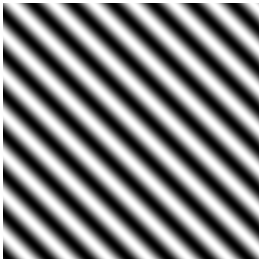
\includegraphics[angle=0,width=0.3\textwidth]{images/wsignal}}\hspace{1em}
    \subfloat[Small amplitude (with orientation perpendicular to the pattern)]{\label{stssignal}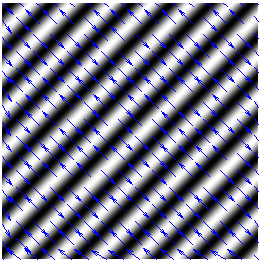
\includegraphics[angle=0,width=0.3\textwidth]{images/stssignal}}\hspace{1em}
    \subfloat[Superimposed image]{\label{mixsignal}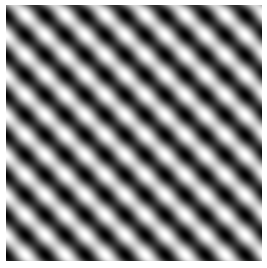
\includegraphics[angle=0,width=0.3\textwidth]{images/mixsignal}}\\
    \subfloat[Coherency for small amplitude]{\label{cwsignal}
\includegraphics[angle=0,width=0.3\textwidth]{images/cwsignal}}\hspace{1em}
    \subfloat[Orientation for the superimposed image (perpendicular to the stronger pattern)]{\label{stmixsignal}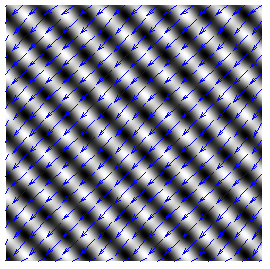
\includegraphics[angle=0,width=0.3\textwidth]{images/stmixsignal}}\hspace{1em}
    \subfloat[Coherency for superimposed image]{\label{cmixsignal}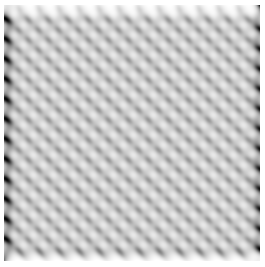
\includegraphics[angle=0,width=0.3\textwidth]{images/cmixsignal}}
    \caption[]{Two patterns being superimposed. Note that even though
    the amplitude visually seems to be the same, they \emph{are}
    different. MATLAB insists on correcting the colors. The image in
    \textbf{fig. \ref{mixsignal}} is the addition of images in
    \textbf{\ref{wsignal} and \ref{stssignal}}. The two patterns are
    ideally oriented in different directions. \textbf{Fig.
    \ref{cwsignal}} shows the coherency for the weak pattern. Note that
    the orientation for the superimposed image corresponds to the
    orientation of the stronger pattern (\textbf{fig. \ref{stmixsignal}}).}
    \label{superimposed}
\end{figure}
\clearpage

\subsection*{Question 6.2}
In determining the structure tensor I have used the MATLAB code supplied
by Gopal from \citep{nonlindiff}. The method \texttt{g = gD(fs, scale,
ox, oy)}\footnote{One should note that you need to swap $x$ and
$y$ in order to produce the expected results.} is the only one used from
the package to calculate derivatives in the image.

The following definition for the structure tensor is used
\begin{equation}
    S = G_\sigma \star \left[\begin{array}{c c}
        I_xI_x & I_xI_y \\
        I_xI_y & I_yI_y
    \end{array}
    \right]
    \label{struct_tensor_def}
\end{equation}
where $I_p$ is the first order derivative in the p-direction. Thus,
$I_xI_x = I_x^2$ is pointwise multiplication of the first order
derivative in the x-direction.

Now, for each pixel in the original image we have a $2\times2$ matrix
like that given in eq. \eqref{struct_tensor_def}. To find the direction
of the structure tensor it is said in \citep[p. 366]{jahne-digital} that
\emph{the eigenvector to the maximum eigenvalue gives the orientation
of the local neighbourhood}. We then find the eigenvalues and
eigenvectors of $S$ for each pixel giving the orientation for the local
neighbourhood.

A figure illustrating the orientation of the structure tensor is shown
in fig. \ref{structure_tensors}. The MATLAB-code is included in the
appendix as the method \texttt{StructureTensor}. The code for the actual
plot of the structure tensor is included in the file
\texttt{assignment621.m}.

\begin{figure}[!h]
    \centering
    \subfloat[Dominant eigenvector.]{\label{structure_tensor_0}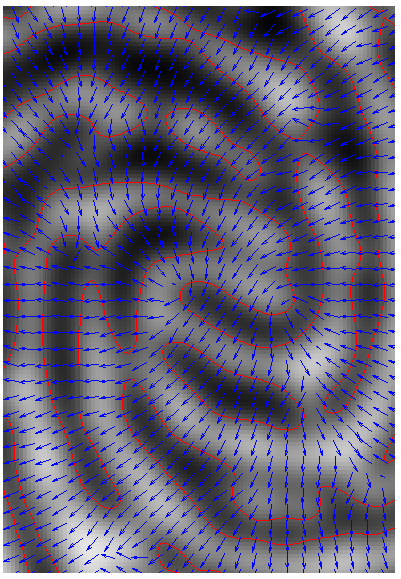
\includegraphics[angle=0,width=0.45\textwidth]{images/structure_tensor_0}}\hspace{1em}
    \subfloat[Non-dominant eigenvector (normal to the dominant).]{\label{structure_tensor_1}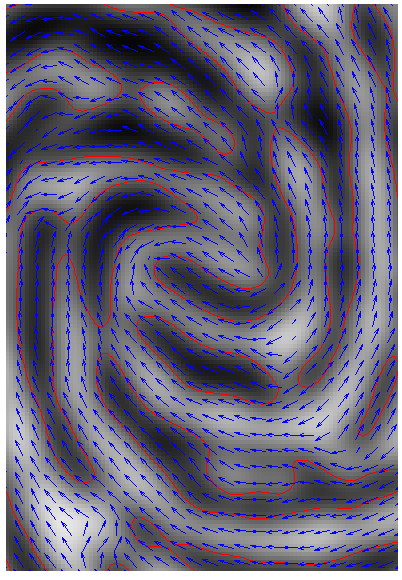
\includegraphics[angle=0,width=0.45\textwidth]{images/structure_tensor_1}}\\
    \caption[]{The structure tensor. The left image shows the
    orientation of the local neighbourhood by the dominant eigenvector.
    The arrows seems a bit messy, but when you look at the normal, i.e.
    the non-dominant eigenvector, then you see that we find the structure
    in the image nicely. Actually, the direction here is always
    perpendicular to the contour lines in the image, thus the other
    eigenvector is parallel to the contour lines.}
    \label{structure_tensors}
\end{figure}

\begin{figure}[!h]
    \centering
    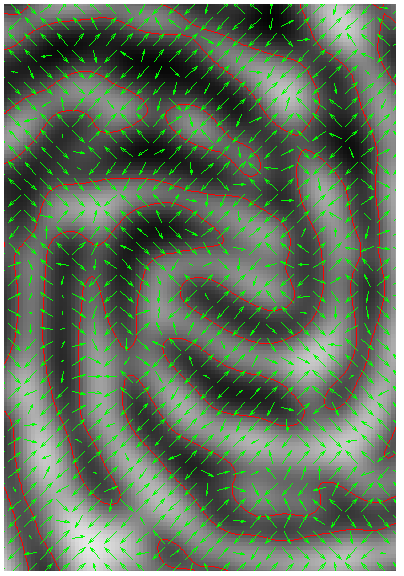
\includegraphics[angle=0,width=0.45\textwidth]{images/gradient_vector}
    \caption[]{The gradient direction. Arrows point towards white and is
    somewhat perpendicular to the red contour line.}
    \label{gradient_vector}
\end{figure}

Comparing the structure tensor and the gradient direction we see that
the gradient always points towards white and is almost perpendicular to
contour lines. The structure tensor is always perpendicular to the
contour lines, but do not necessarily point towards white. This is
because the structure tensor look at the neighbourhood rather than just
the gradient. It it interesting to see how well we actually find the
structure in the image using the structure tensor.

With respect to the actual image, that of a fingerprint, we can
determine the shape of the filter used for image enhancement by using
the structure tensor. We want to preserve the dominant edges, thus do
not want to blur these edges. The structure tensor have just found these
edges (or ridges).

\clearpage

%%%%%%%%%%%%%%%%%%%%%%%%%%%%%%%%%%%%%%%%%%%%%%%%%%%%%%%%%%%%%%%%%%%%
% Formal stuff

\bibliographystyle{abbrvnat}
\bibliography{bibliography}
%\addcontentsline{toc}{chapter}{Litteratur}

\appendix
\lstset{language=Matlab, basicstyle=\scriptsize,
    showstringspaces=false, numbers=left, stepnumber=1,
    numberstyle=\tiny, frame=none}
\section{Source code}

\subsection{assignment611.m}
\lstinputlisting{../../src/assignment611.m}

\subsection{assignment621.m}
\lstinputlisting{../../src/assignment621.m}

\subsection{StructureTensor.m}
\lstinputlisting{../../src/StructureTensor.m}

\subsection{GradientVector.m}
\lstinputlisting{../../src/GradientVector.m}

\end{document}

% vim: set tw=72 spell spelllang=en:
